\documentclass{beamer}
\usetheme{Darmstadt}
\usecolortheme{beaver}
\usepackage{booktabs}

\usepackage[utf8]{inputenc}
\usepackage{graphicx}
\graphicspath{ {./images/} }


%Information to be included in the title page:
\title{Homework 1 Presentation}
\author{Brandon Hosley}
\institute{University of Illinois - Springfield}
\date{\today}

\begin{document}
\frame{\titlepage}

\begin{frame}{Overview}
\tableofcontents
\end{frame}

\section{Supervised and Unsupervised Learning}
\begin{frame}{Supervised and Unsupervised Learning}
	\begin{itemize}%[<+->]
		\item[Q:] What's the difference between Supervised and Unsupervised learning? \\
		%\item[A:] Supervised training data is \emph{well} labeled, with \emph{ground truth}.
	\end{itemize}
\end{frame}

\begin{frame}{Supervised and Unsupervised Learning}
	\begin{columns}
	\column{0.5\textwidth}
	Supervised Learning
		\begin{itemize}
			\item<1-> Labeled Data
			\item<2-> Known Features
			\item<3-> Leverages Experience
		\end{itemize}
	
	\column{0.5\textwidth}
	Unsupervised Learning
		\begin{itemize}
			\item<1-> Unlabeled Data
			\item<2-> Unknown Features
			\item<3-> Discovers New Patterns
		\end{itemize}
	\end{columns}
	\only<1-3>{
		\begin{block}{Remark}
			\only<1>{Supervised learning requires labeled or pre-classified data.}
			\only<2>{Labeled data implies that the feature of interest is already known.}
			\only<3>{Supervised learning will model already established patterns;
				unsupervised may discover new patterns, or new ways to group or cluster data.}
		\end{block}}
	\only<1>{
		\begin{alertblock}{Caution!}
			Labeled data often comes with a greater up-front cost, typically through manual classification. 
		\end{alertblock}}
	\only<2>{
		\begin{exampleblock}{Examples:}
			$\cdot$ Training a model to classify pictures of animals \\
			$\cdot$ Training a model for handwriting recognition
		\end{exampleblock}}
	\onslide<4>{\centering 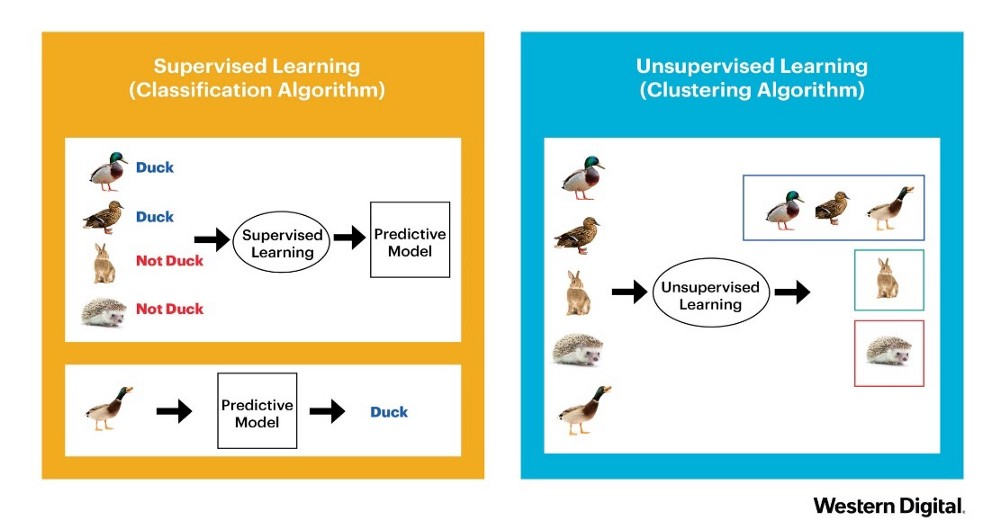
\includegraphics[width=0.95\linewidth]{SupVsUnsup} }
\end{frame}

\begin{frame}{Common Uses: Supervised Learning}
	\begin{columns}
		\column{0.5\textwidth}
		Supervised Learning
		\begin{itemize}
			\item<1-> Predictive Modeling
			\item<2-> Classification
			\item<3-> Regression
		\end{itemize}
		
		\column{0.5\textwidth}
		\only<1>{\begin{block}{Remark} Using known data to predict results \end{block}}
		\only<2>{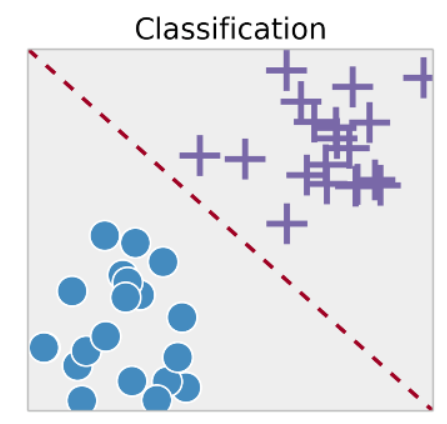
\includegraphics[width=0.75\linewidth]{SupClassification}}
		\only<3>{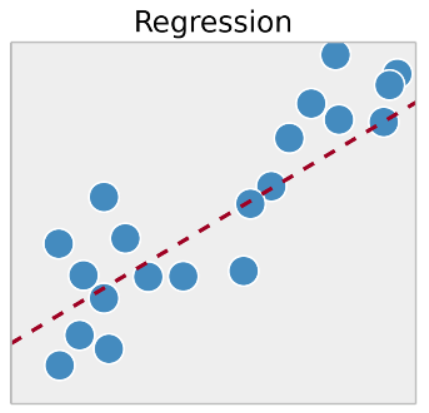
\includegraphics[width=0.75\linewidth]{SupRegression}}
	\end{columns}
	\includegraphics<1>[width=\linewidth]{SupPredictiveModeling}
	\begin{block}<2->{Remark}
			\only<2>{Classification into known group types based on the features provided to the model}
			\only<3>{Regression analysis based on the provided data}
		\end{block}
\end{frame}

\begin{frame}{Common Uses: Unsupervised Learning}
	\begin{columns}
		\column{0.5\textwidth}
		\only<1> Unlabeled Data
		\only<2> Unknown Features
		\only<3> Discovers New Patterns
		
		\column{0.5\textwidth}
		Unsupervised Learning
		\begin{itemize}
			\item<1-> Labeled Data
			\item<2-> Known Features
			\item<3-> Leverages Experience
		\end{itemize}
	\end{columns}
\end{frame}

\begin{frame}{Adversarial Networks: The Happy Medium?}

\end{frame}

%%----------------------------------------------------------------------------------%%
\section{Hastie and Tibshirani}

\begin{frame}{Hastie and Tibshirani}

\end{frame}

\end{document}
